\chapter{传输链路}
安全链路支持3种传输协议:QUIC协议、WebSocket协议和WebTransport协议。
本章节主要说明链路传输中所使用的协议,并分析它们的安全性和可靠性。

\section{QUIC协议}
QUIC是一个通用的基于UDP协议的传输层网络协议,最初由Google设计实现并大规模部署\cite{langley2017quic},该协议旨在解决TCP协议的许多问题,减少客户端服务器连接的延迟。
2021年,其于RFC 9000\cite{rfc9000}中正式推出标准化版本。
QUIC与HTTP/2的多路复用连接协同工作,允许多个数据流独立到达所有端点,因此不受涉及其他数据流的丢包影响。
QUIC的次要目标包括降低连接和传输时延,以及每个方向的带宽估计以避免拥塞。
HTTP/3是即将到来的第三个主要版本的HTTP协议,将基于QUIC协议实现,在RFC 9114\cite{rfc9114}得到标准化。
另外,DoQ(DNS over QUIC)也处于研究阶段。

\begin{figure}[H]
  \centering
  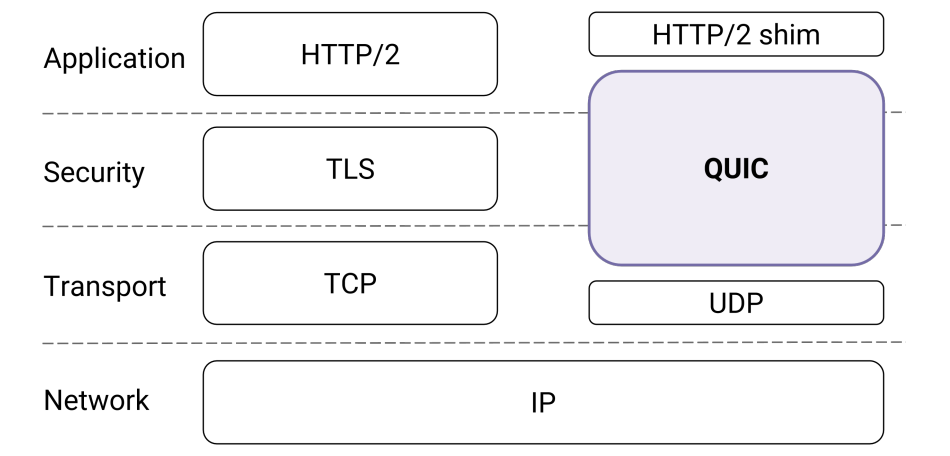
\includegraphics[width=\textwidth]{quic}
  \caption{传统HTTPS堆栈与QUIC的对比}
\end{figure}

\subsection{可靠加密隧道}
由于QUIC基于TLS1.3,因此客户端和服务器在传输数据前先要经过密钥协商握手,之后双方通信的数据都经过共同协商的密钥加密传输。
TLS握手后,通信双方建立起一条安全的加密隧道。TLS 1.3采用的AEAD加密算法,保证了认证加密(Authenticated encryption),这是一种能够同时保证数据的保密性、完整性和真实性的一种加密模式。
本课题选用了其中的TLS\_CHACHA20\_POLY1305\_SHA256作为通信双方使用的加密算法。

\subsection{低延迟}
相较于TLS/TCP,建立在QUIC的安全连接有低延迟的优点。
使用TLS/TCP,通信双方建立一条安全连接,需要经过TCP3次握手和
TLS 1.2握手共消耗3次往返时间(RTT)。尽管有TCP Fast Open\cite{radhakrishnan2011tcp}和TLS1.3可以改进,但需要额外的配置,在实际部署也有许多问题。
而使用QUIC初次建立安全连接,需要1-RTT,之后甚至只需要0-RTT,意味着数据可以不需要等待TLS1.3握手结束直接发送。

\section{WebSocket协议}
WebSocket是一种网络传输协议,可在单个TCP连接上进行全双工通信,位于OSI模型的应用层。
WebSocket协议由IETF在2011年作为RFC 6455\cite{rfc6455}进行了标准化,当前允许Web应用程序使用该协议的API规范称为WebSockets。
WebSocket使得客户端和服务器之间的数据交换变得更加简单,允许服务端主动向客户端推送数据。
在WebSocket API中,浏览器和服务器只需要完成一次握手,两者之间就可以创建持久性的连接,并进行双向数据传输。

\begin{figure}[H]
  \centering
  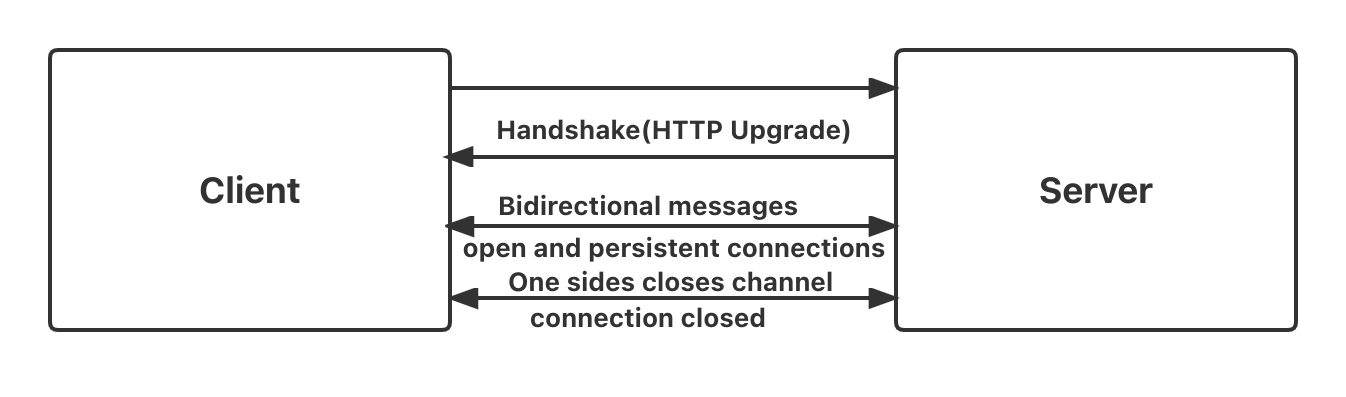
\includegraphics[width=\textwidth]{websocket}
  \caption{WebSocket协议有两部分:建立升级连接的握手,然后是实际的数据传输。
  首先,客户端通过使用Upgrade:WebSocket和Connection:Upgrade头字段以及一些特定于协议的头字段来请求WebSocket连接。 
  如果服务器支持该协议,则回复相同的 Upgrade: WebSocket 和 Connection: Upgrade头字段并完成握手。
  一旦握手成功完成,客户端和服务器就建立了全双工通信,任意一方可以结束WebSocket连接。}
\end{figure}

\begin{figure}[H]
  \centering
  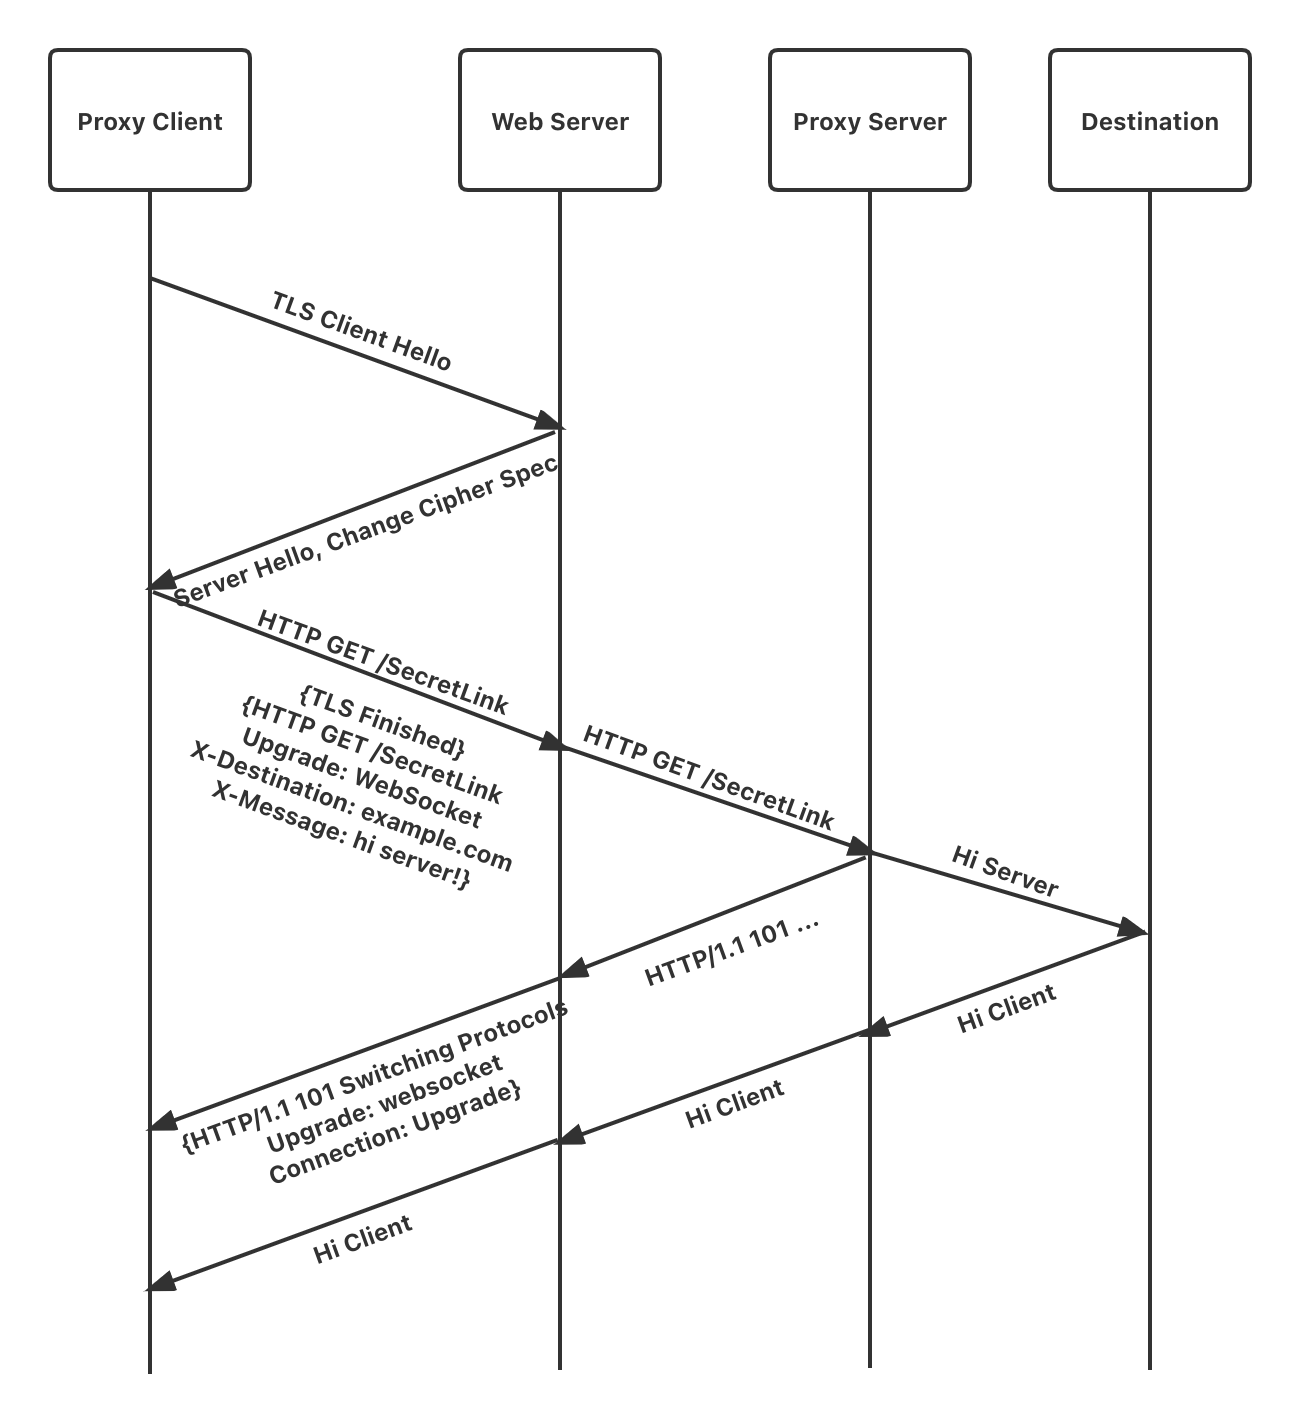
\includegraphics[width=\textwidth]{websocket_proxy}
  \caption{基于WebSocket的加密隧道通信双方握手过程}
\end{figure}

\section{WebTransport协议}
WebTransport是一种使用HTTP/3协议的应用层网络传输协议,它旨在用于Web客户端和HTTP/3服务器之间的双向通信。 
它可以像WebSockets一样使用,但支持单向通信和双向通信、无序的数据传输以及可靠和不可靠的传输。

\section{特点}
分析研究了基于WebSocket/WebTransport的加密通信隧道特点:

\subsection{秘密URL}
本课题中,设置秘密URL为一个随机生成的UUID,客户端可以包含共享的初始HTTP请求的URL中的秘密作为身份验证机制。 
Web服务器配置为反向将所有访问秘密URL的请求代理到下一跳节点,而其他的HTTP请求返回正常的HTTP响应。

\subsection{重放攻击保护}
T需要客户端在一个特定的URL(一个事先共享的UUID)下与服务器建立WebSocket连接,并且这些发生在TLS1.3握手后(保证了加密)。
这允许Web服务器以正常的方式响应错误页面(例如正常的HTML页面或者404 Not Found),与非代理网络服务器没有区别。 
因此,只要攻击者无法得知共享秘密,在应用层协议的共享秘密可以避免重放攻击。

\subsection{Web服务器伪装}
利用现有的网络服务器,方便部署,同时使加密流量更难挑出或识别。
我们可以将代理隐藏在真实的Web服务器后面,例如Nginx、Caddy,无需模仿TLS协议。

\subsection{额外开销}
在最初的TCP(WebTransport不需要)和 TLS 握手之后,加密隧道的开销是很小的。
为了避免发送与 HTTP 兼容的编码相关的开销,改为在客户端和服务器之间使用WebSocket(基于TCP)或WebTransport(基于QUIC)。
这允许客户端和服务器通过Web服务器发送二进制数据,同时避免需要额外的 HTTP 安全编码,例如 MIME 或base 64。

\subsection{使用流行的协议}
先前的工作表明,加密流量可以使用熵分析和机器学习等方式检测。
在加密隧道中,我们依靠流行的TLS协议来传输数据,这使得对流量的分析很困难,并且难以受到由于协议的特殊性导致的指纹攻击。

\subsection{局限性}
使用WebSocket或WebTransport作为传输协议需要真实的Web服务器,需要一个真实的域名(DNS解析到目标服务器),
部署代价比直接使用QUIC要高。


\section{性能比较}
针对三种通信协议,分别比较从一个节点到另一个节点的一跳的传输延迟、上传速率和下载速率,结果如下:

\subsection{传输延迟}
比较三种传输方式的传输延迟,QUIC和WebTransport的传输延迟基本相同,WebSocket的传输延迟较高一点。

\begin{table}[H]
  \begin{tabular}{|c|c|c|c|c|c|}
  \hline
  传输协议 & 平均延迟 & 最低延迟 & 最高延迟 & 延迟中位数 & 延迟平均差值  \\ \hline        
  QUIC & 226.08ms & 215.2ms & 273.6ms & 221.5ms & 14.2ms \\ \hline    
  WebSocket & 264.24ms & 252.1ms & 328.8ms & 256.7ms & 19.1ms \\ \hline          
  WebTransport & 232.95ms & 218ms & 296.6ms & 223.3ms & 20.3ms \\ \hline         
  \end{tabular}
  \caption{比较三种传输方式的传输延迟,20次测试的结果。}
\end{table}

\begin{figure}[H]
  \centering
  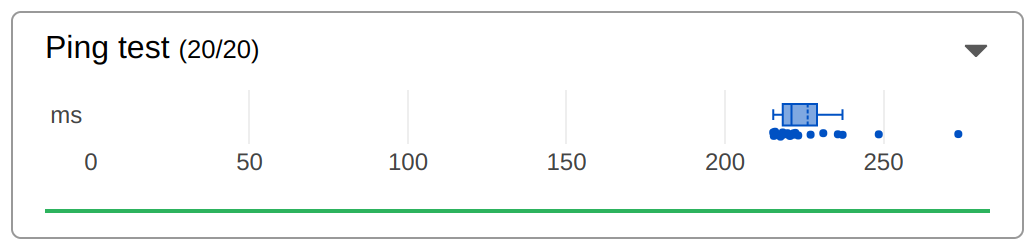
\includegraphics[width=\textwidth]{ping_quic}
  \caption{基于QUIC的加密隧道}
\end{figure}

\begin{figure}[H]
  \centering
  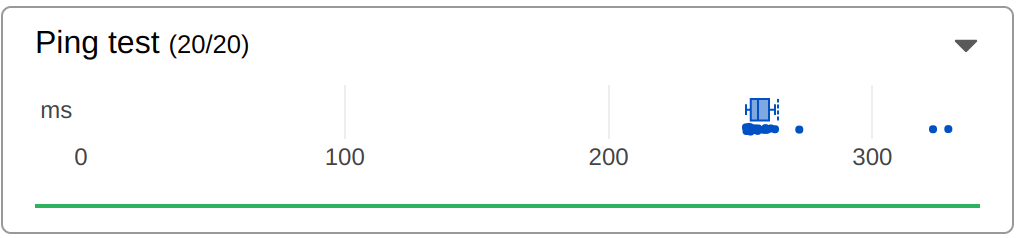
\includegraphics[width=\textwidth]{ping_websocket}
  \caption{基于WebSocket的加密隧道}
\end{figure}

\begin{figure}[H]
  \centering
  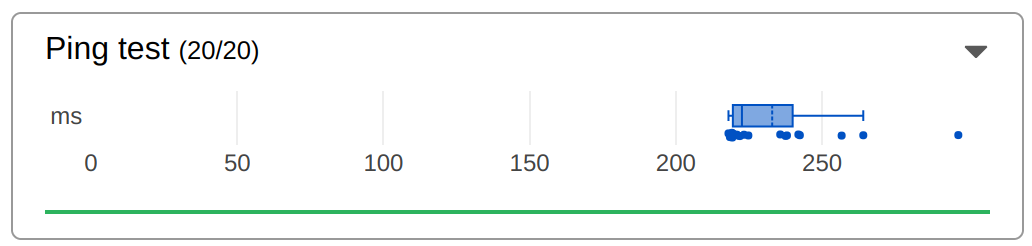
\includegraphics[width=\textwidth]{ping_webtransport}
  \caption{基于WebTransport的加密隧道}
\end{figure}


\subsection{下载速率}
比较三种传输方式的下载速率,WebSocket和WebTransport的下载速率基本相同,QUIC的下载速率更低一点。

\begin{table}[H]
  \begin{tabular}{|c|c|c|c|c|}
  \hline
  传输协议 & 平均下载速率 & 最低下载速率 & 最高下载速率 & 下载速率中位数  \\ \hline        
  QUIC & 10.33Mbps & 8.52Mbps & 13.82Mbps & 9.73Mbps \\ \hline    
  WebSocket & 18.58Mbps & 2.32Mbps & 21.7Mbps & 21.2Mbps \\ \hline          
  WebTransport & 21Mbps & 9.75Mbps & 24.98Mbps & 23.8Mbps \\ \hline         
  \end{tabular}
  \caption{下载1MB大小的文件,8次测试的结果。}
\end{table}

\begin{figure}[H]
  \centering
  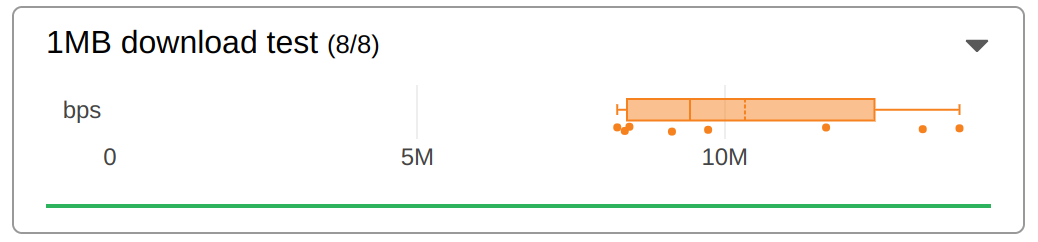
\includegraphics[width=\textwidth]{download_quic}
  \caption{基于QUIC的加密隧道}
\end{figure}

\begin{figure}[H]
  \centering
  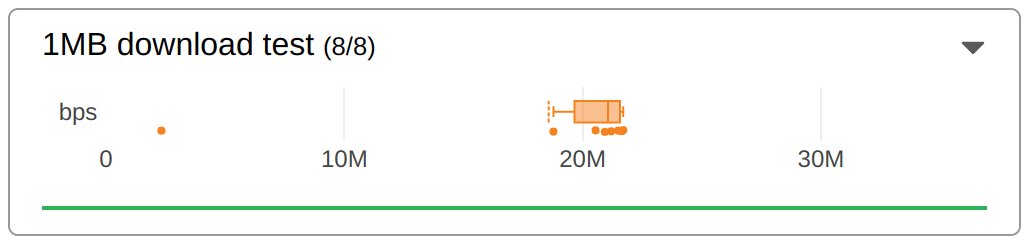
\includegraphics[width=\textwidth]{download_websocket}
  \caption{基于WebSocket的加密隧道}
\end{figure}

\begin{figure}[H]
  \centering
  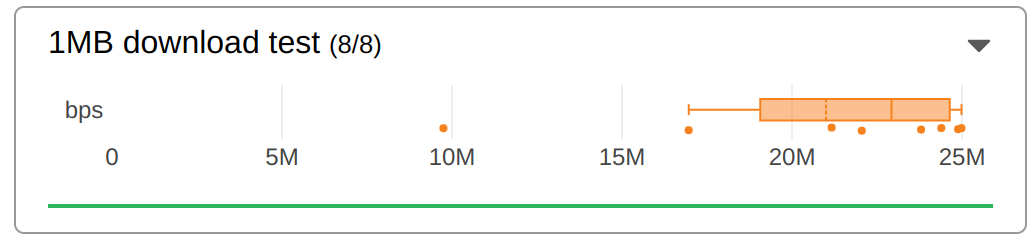
\includegraphics[width=\textwidth]{download_webtransport}
  \caption{基于WebTransport的加密隧道}
\end{figure}


\subsection{上传速率}
比较三种传输方式的上传速率,QUIC和WebTransport的上传速率基本相同,WebSocket的上传速率更高一点。

\begin{table}[H]
  \begin{tabular}{|c|c|c|c|c|}
  \hline
  传输协议 & 平均上传速率 & 最低上传速率 & 最高上传速率 & 上传速率中位数  \\ \hline        
  QUIC & 1.29Mbps & 930.91kbps & 1.93Mbps & 1.07Mbps \\ \hline    
  WebSocket & 3.03Mbps & 2.72Mbps & 3.72Mbps & 2.91Mbps \\ \hline          
  WebTransport & 1.14Mbps & 660.55kbps & 1.61Mbps & 1.3Mbps \\ \hline         
  \end{tabular}
  \caption{上传1MB大小的文件,6次测试的结果。}
\end{table}

\begin{figure}[H]
  \centering
  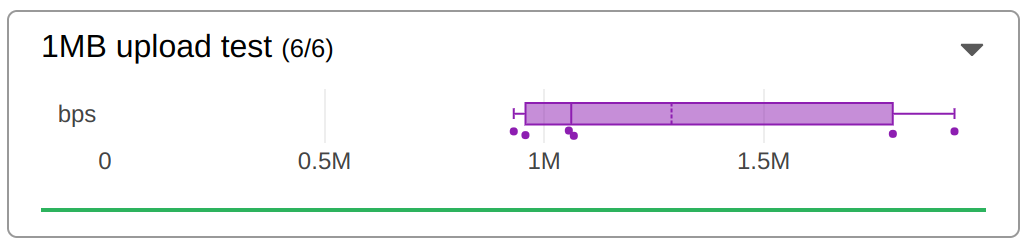
\includegraphics[width=\textwidth]{upload_quic}
  \caption{基于QUIC的加密隧道}
\end{figure}

\begin{figure}[H]
  \centering
  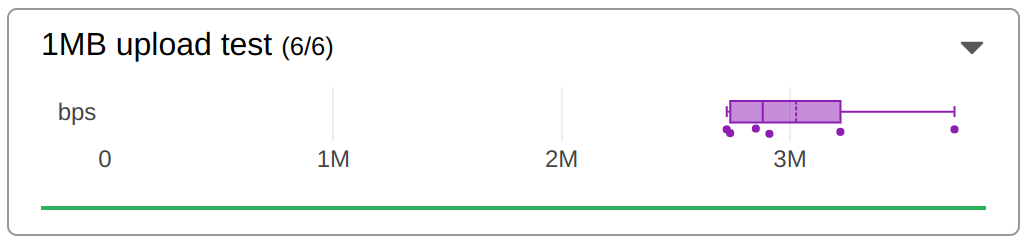
\includegraphics[width=\textwidth]{upload_websocket}
  \caption{基于WebSocket的加密隧道}
\end{figure}

\begin{figure}[H]
  \centering
  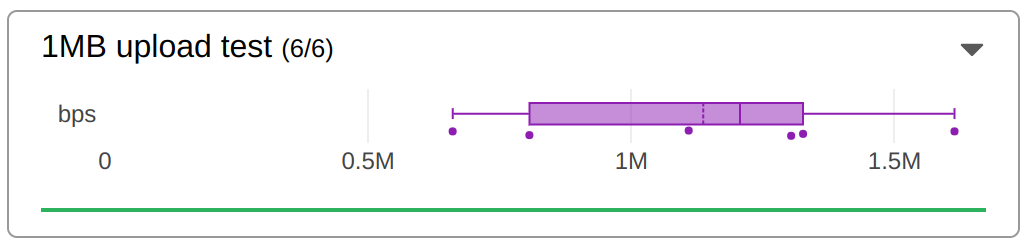
\includegraphics[width=\textwidth]{upload_webtransport}
  \caption{基于WebTransport的加密隧道}
\end{figure}

\section{三种协议对比分析}
本课题中,在加密隧道的传输协议实现了QUIC、WebSocket和WebTransport,三种协议有着各自的优缺点。
下面是基于QUIC、WebSocket、WebTransport的加密隧道比较:

\subsection{基于QUIC的加密隧道}
相较于基于WebSocket和WebTransport的加密隧道,基于QUIC的加密隧道的延迟和传输速率会更好。
由于底层基于传输层的QUIC协议而非应用层的HTTP协议,不需要第一步的HTTP请求就能直接与目标建立加密连接,因此在延迟上会少1RTT。

相较于基于WebSocket和WebTransport的加密隧道,基于QUIC的加密隧道提供了更好的便捷性。
在配置上有更高的自由度,不需要一个真实的域名(DNS解析到目标服务器),部署代价要更低。

\subsection{基于WebSocket的加密隧道}
相较于基于QUIC的加密隧道,基于WebSocket的加密隧道提供了更好的流量混淆。
因为数据传输通过真实并且广泛使用的协议(WebSocket),对于未知的连接也会返回正常的网页服务器响应,如一个正常的HTML页面或者404 Not Found。
同时,基于WebSocket的加密隧道可以很容易的适用于现有的网页服务器(Nginx、Caddy等),只需要设置反向代理特定的UUID对应的路由到加密隧道节点就可以完成(在配置文件上添加几行代码)。

相较于基于WebTransport的加密隧道,基于WebSocket的加密隧道提供了更好的便捷性。
目前WebSocket已经被广泛使用,许多反向代理服务器如Nginx、Caddy都包含对WebSocket的支持,因此部署和使用更加方便。

\subsection{基于WebTransport的加密隧道}
相较于基于QUIC的加密隧道,基于WebTransport的加密隧道提供了更好的流量混淆。
因为数据传输通过真实的协议(WebTransport),对于未知的连接也会返回正常的网页服务器响应,如一个正常的HTML页面或者404 Not Found。

相较于基于WebSocket的加密隧道,基于WebTransport的加密隧道底层的QUIC协议解决了TCP队头阻塞的问题,其延迟和传输速率会更好。
然而,由于WebTransport目前还处在草案阶段,没有大规模部署和流行,因此成熟度上没有WebSocket好。
